\documentclass[IAHR]{IAHR}

%%%%%%%%%%%%%%%%%%%%%%%%%%%%%%%%%%%%%%%%%%%%%%%%%%%%%%%
% Packages
\usepackage{array}
\usepackage{graphicx}
\usepackage[utf8]{inputenc}

%%%%%%%%%%%%%%%%%%%%%%%%%%%%%%%%%%%%%%%%%%%%%%%%%%%%%%%
% Header
\title{ABSRACT TITLE}
\author[*1]{Presenting Author}
\author[1,2]{Second Author}
\author[2]{Third Author}

\affil[1]{Department name, Institution 1} 
\affil[2]{Department name, Instituion 2} 
% corresponding/presenting author email
\corrauthor{correspondingauthor@email.com}

%%%%%%%%%%%%%%%%%%%%%%%%%%%%%%%%%%%%%%%%%%%%%%%%%%%%%%%
\begin{document}

\maketitle

Enter your abstract here. Ensure that your document is no longer than 1 page in length. It is a good idea to start your abstract with some background and motivation, then describe your approach and summarize the key results.

We recommend adding an eye-catching figure.  Just make sure that the total length of the abstract is no more than 1 page.

\begin{figure}[htpb!]
\begin{center}
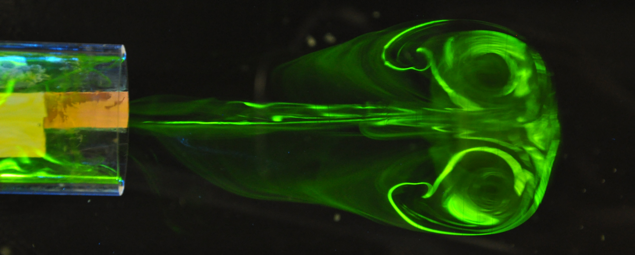
\includegraphics[scale=1]{vortex_ring.pdf}
\caption{Sample figure provided by Katherine Grayson.}
\label{Fig}
\end{center}
\end{figure}

Any references should appear together at the end of the abstract, listed alphabetically by last name of the first author. Cite in the text using commands \citep{gargett1984,lilly1983} or \cite{thorpe2005}. 

%%%%%%%%%%%%%%%%%%%%%%%%%%%%%%%%%%%%%%%%%%%%%%%%%%%%%%%
\bibliographystyle{IAHR}
\bibliography{IAHR}

\end{document}